\documentclass[11pt]{article} % article, report, or book

\usepackage[margin=1.0in]{geometry}
%\usepackage[parfill]{parskip}    		% Activate to begin paragraphs with an empty line rather than an indent
\usepackage{graphicx}				% Use pdf, png, jpg, or eps§ with pdflatex; use eps in DVI mode
\graphicspath{{../figures/}}
\usepackage{amsmath, bm}
\usepackage{color}
\usepackage[utf8]{inputenc} % allows for é
\usepackage{float} % allows for [H]
\usepackage{booktabs, caption, makecell}
\renewcommand\theadfont{\bfseries}
\usepackage{setspace}

%==================================================================
\title{A Discussion of Homoclinic Orbits in the Circular Restricted Three-Body Problem}
\author{Luke Bury \& Don Kuettel}
%==================================================================
\begin{document}
\maketitle
%==================================================================
\section{Introduction}
In 1885, a competition was held by Acta Mathematica in which participants were challenged to solve one of four outstanding math problems. Henri Poincaré, a prominent mathematician of the time, entered the contest and ultimately won. However, his submission contained a critical mistake that, when corrected, led to the discovery of homoclinic orbits. In mathematics, a homoclinic orbit is defined as a trajectory which joins a saddle equilibrium point to itself. More precisely, a homoclinic orbit is a union between the stable manifold, $W^s(p)$, and the unstable manifold, $W^u(p)$, of an equilibrium point. Figure \ref{f:homoclinic_example} shows an example of a simple, two-dimensional homoclinic orbit about the saddle equilibrium point $p$. As the figure shows, as time approaches either negative or positive infinity, the homoclinic orbit will approach $p$. 

\begin{figure}[H]
    \centering
    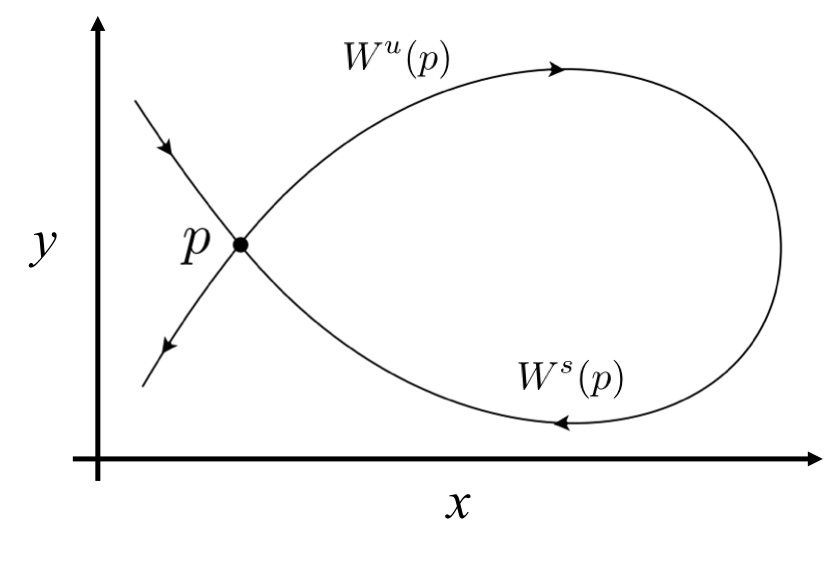
\includegraphics[width=4in]{homoclinic_orbit.png}
    \caption{A 2-Dimensional homoclinic orbit.}
    \label{f:homoclinic_example}
\end{figure}

Homoclinic orbits can reveal much about the chaotic behavior of dynamical systems, but locating these orbits requires a non-trivial, multi-step process. First, a periodic orbit about a chosen equilibrium point must be identified. From this periodic orbit, both stable and unstable manifolds must be constructed. Finally, intersections of the stable and unstable manifolds are found via Poincaré sections, and homoclinic orbits are thus identified. The following report briefly discusses the history of Poincare's discovery of homoclinic orbits and demonstrates a detailed procedure for locating these orbits. Ultimately, homoclinic orbits in the Earth-Moon system are found and presented.

\section{The Competition}
As documented by Andersson and Barrow-Green \cite{Andersson1994,BarrowGreen1994}, in 1885, Acta Mathematica announced a mathematics competition to the world. This competition, sponsored by King Oscar II of Sweden, encouraged interested parties to make an attempt at solving one of four unanswered problems of the time. Henri Poincaré, a prominant mathematician (who was largely favored to win the competition) attempted the first problem, which essentially asked for a solution to the perplexing $n$-body problem. Rather than sticking to the exact prompt, Poincaré decided to instead attempt a subset of the $n$-body problem known as the three-body problem - the first order of the $n$-body problem remaining unsolved. To further simplify his initial effort, Poincaré restricted the three-body system in a manner known today as the Circular Restricted Three-Body Problem (CR3BP), which will be discussed further in the next section.

Poincaré's submission to the competition was the culmination of several strands of his work from the previous decade, which included geometrical and analytical theory, integral invariants, and periodic solutions to dynamical systems. Poincaré applied these theories in an attempt to rigorously prove stability and find periodic solutions for the CR3BP. The competition judges immediately recognized the importance of Poincaré's submission and unanimously crowned him the victor. However, around the time that his work was first being printed, a discussion with Lars Edvard Phragmén led to the discovery of an error within Poincaré's submission that held significant ramifications. The error was rooted in Poincaré's failing ``to take proper account of the exact geometric nature of a particular curve'' \cite{BarrowGreen1997}. In Theorem III of the paper's first, and flawed, edition, Poincaré claimed that a particular invariant curve was closed (Figure \ref{fig:curveIntersection1}(a,b)). He failed to consider that the curve could be self-intersecting (Figure \ref{fig:curveIntersection1}(c)). After realizing his mistake, Poincaré reworked his derivations to discover that the asymptotic surfaces are not closed, but instead, they intersect along infinitely many asymptotic trajectories. Ironically, this mistake cemented Poincaré's place among legendary mathematicians for his resulting discovery of \textit{doubly asymptotic}, or \textit{homoclinic}, points/orbits in the CR3PB and dynamical systems in general. These curves will resurface in section \huge\color{red}\textbf{???????}\color{black}\normalsize as the Poincaré sections of intersecting stable and unstable manifolds, where exact intersections of the curves correspond to homoclinic orbits. First, however, the CR3BP and periodic orbits must be well understood.

\begin{figure}[H]
\centering
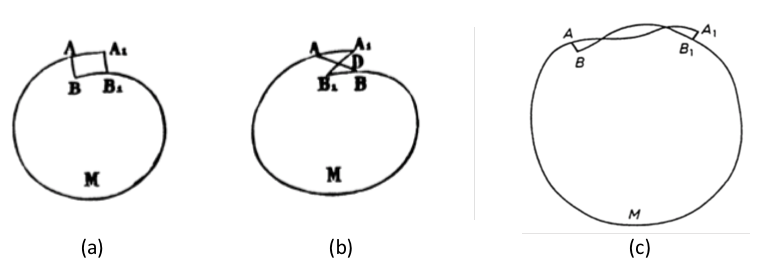
\includegraphics[width=5in]{curveIntersection1.png}\nonumber{}
\caption{(a) Diagrams of incorrectly closed invariant curves from the first edition of Poincaré's memoir. (b)Invariant curve with self intersection from Poincaré's corrected work \cite{BarrowGreen1997}.}
\label{fig:curveIntersection1}
\end{figure}

%-------------------------------------------------------------------
%-------------------------------------------------------------------
\section{Circular Restricted Three Body Problem}
Before studying periodic orbits, their manifolds, and the process of locating homoclinic orbits, it is necessary to provide the reader a solid foundation of the Circular Restricted Three Body Problem (CR3BP) - the dynamical system in which the aforementioned trajectories are created and analyzed. In the CR3BP (Fig. \ref{f:CR3BP}), the origin of the system is set at the barycenter of the two main bodies in the system (e.g., the Earth \& Moon), and the frame rotates so these bodies remain stationary on the x-axis. The bodies are assumed to move in perfectly circular orbits and act as point masses from a gravitational perspective. The restricted problem is then to ascertain the motion of the third body whose mass is considered negligible. The system is typically normalized so that the masses of the two primary bodies sum to 1 (i.e., $m_1 = \mu$ and $m_2 = 1-\mu$, where $\mu = m_2/(m_1+m_2)$ is known as the three-body parameter), the distance between the primaries is 1, the orbital period period of the primaries is $2\pi$, and the gravitational constant G is equal to 1. Under these conditions, the equations of motion for the CR3BP are shown in Equations \ref{e:eomx}-\ref{e:eomz}:

\begin{align}
	\ddot{x} &= 2\dot{y} + x - (1-\mu)\left(\dfrac{x+\mu}{r_1^3}\right) - \mu\left(\dfrac{x-1+\mu}{r_2^3}\right) \label{e:eomx}\\
	\ddot{y} &= -2\dot{x} + y\left(-\dfrac{1-\mu}{r_1^3} - \dfrac{\mu}{r_2^3} + 1\right) \label{e:eomy}\\
	\ddot{z} &= z\left(-\dfrac{1 - \mu}{r_1^3} - \dfrac{\mu}{r_2^3}\right), \label{e:eomz}
\end{align} 

\noindent
where

\begin{align}
	r_1 & = \sqrt{\left(x + \mu\right)^2 + y^2 + z^2} \\
	r_2 & = \sqrt{\left(x - 1 + \mu\right)^2 + y^2 + z^2}.
\end{align}

\begin{figure}[H]
	\centering
	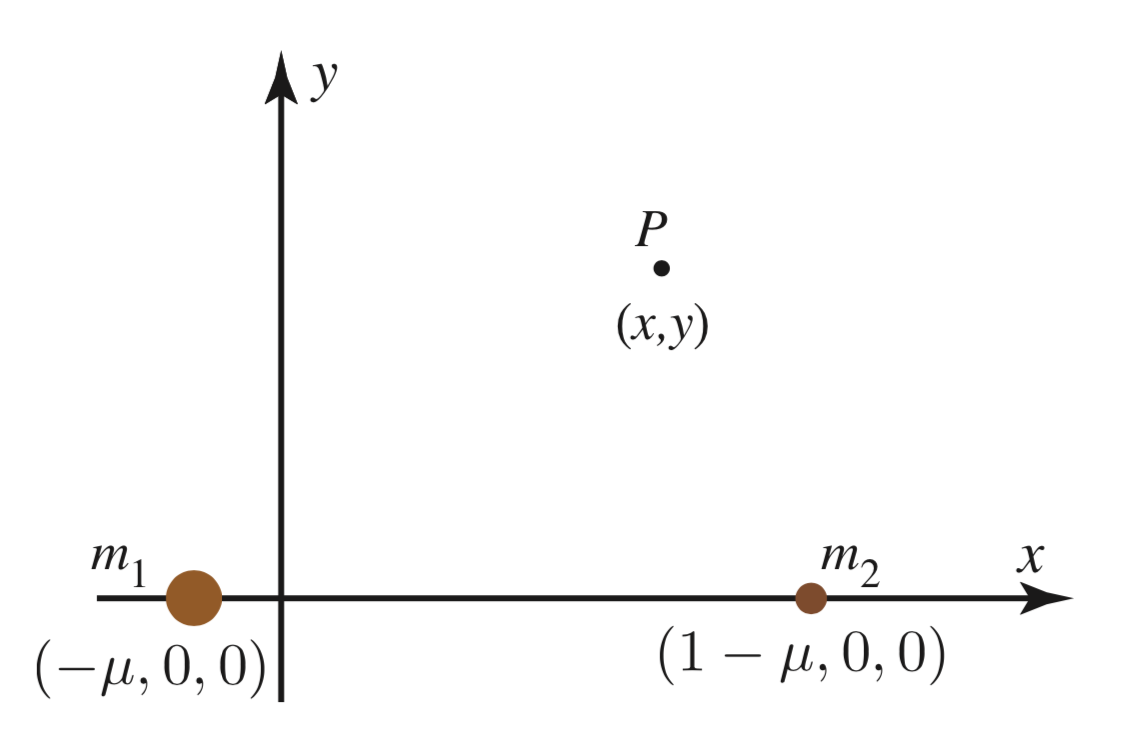
\includegraphics[width=4in]{CR3BP.png}\nonumber
	\caption{This figure shows the layout of the Circular Restricted Three-Body Problem \cite{KoonLoMarsdenRoss2011}.}
	\label{f:CR3BP}
\end{figure}

In most simplified astrodynamic systems (e.g., Keplerian motion, CR3BP, $n$-body porblem, etc...), there are important parameters, known as integrals of motion, that are constant throughout the motion of a system that can be used to define the system. For example, the orbital elements of a trajectory in a Keplerian system are the system's integrals of motion. The integral of motion for the CR3PB is called the Jacobi constant and is given by 

\begin{equation}
	J = -\dot{x}^2-\dot{y}^2-\dot{z}^2+x^2+y^2 + \frac{2\left(1-\mu\right)}{r_1} + \frac{2\mu}{r_2}.
	\label{e:jacobi_constant}
\end{equation}

\noindent
For a given Jacobi constant, the motion of a particle is limited to certain regions of space due to the constraint that the velocity cannot have imaginary components. These restrictive regions, known as zero-velocity curves, are computed by setting the velocity in Equation \ref{e:jacobi_constant} to zero and mapping the resultant surfaces in the CR3PB. The motion of an object with a specific Jacobi constant in bound within its respective zero-velocity curve and can only cross the boundaries under some non-conservative force.

%-------------------------------------------------------------------
\subsection{Equilibrium Point Locations}
Complex dynamical system such as the CR3PB often times have equilibrium points that result in a constant solution to the system's differential equations. In the CR3BP, these points, known as Lagrange points, mark positions where the combined gravitational pull of the two large masses provides precisely the centripetal force required to orbit with them (i.e., the Lagrange points are stationary within the rotating system of the CR3BP). There are five such points labeled L$_1$ - L$_5$ located in the plane of the two primary masses. The first three Lagrange points lie on the line connecting the two primary bodies, and the last two points, L$_4$ and L$_5$, are located at the vertex of an equilateral triangle formed with the two primary bodies \cite{KoonLoMarsdenRoss2011}.

In order to find the location of the five equilibrium points in the CR3BP, the velocity and acceleration must be set to zero in the system's equations of motion. This results in the following equations:

\begin{align}
	0 & = x - (1-\mu)\left(\dfrac{x+\mu}{r_1^3}\right) - \mu\left(\dfrac{x-1+\mu}{r_2^3}\right) \label{e:eomx_zero}\\
	0 & = y\left(-\dfrac{1-\mu}{r_1^3} - \dfrac{\mu}{r_2^3} + 1\right) \label{e:eomy_zero}\\
	0 & = z. \label{e:eomz_zero}
\end{align}

\noindent
If $y$ is set to zero, a quintic equation in $x$ emerges. Solving this equation to first order results in the following location for the first three Lagrange points:

\begin{align}
	L_1 &= \left(1-\left(\frac{\mu}{3}\right)^{1/3},0,0\right)\label{e:L1_loc}\\
	L_2 &= \left(1+\left(\frac{\mu}{3}\right)^{1/3},0,0\right)\label{e:L2_loc}\\
	L_3 &= -\left(1+\left(\frac{5\mu}{12}\right),0,0\right). \label{e:L3_loc}
\end{align}

\noindent
Using Equations \ref{e:L1_loc}-\ref{e:L3_loc} as initial conditions, a Newton-Raphson iteration can then be used to numerically find the exact location of the first three Lagrange points to machine precision. Equations \ref{e:eomx_zero}-\ref{e:eomz_zero} can also be used to find the two triangular equilibrium points, L$_4$ and L$_5$. Since the equilibrium points form an equilateral triangle with the primary bodies, $r_1 = r_2 = 1$ is substituted into Equation \ref{e:eomx_zero} and Equation \ref{e:eomy_zero}. These equations are subsequently solved to provide the exact locations for the remaining equilibrium points:

\begin{align}
	L_4 &= \left(\frac{1}{2}-\mu, \frac{\sqrt{3}}{2},0\right)\\
	L_5 &= \left(\frac{1}{2}-\mu, -\frac{\sqrt{3}}{2},0\right).
\end{align}

\noindent
Using the Earth-Moon CR3BP three-body parameter ($\mu = 0.012155$), Table \ref{t:lagrange_points} shows the non-dimensional locations of the five Lagrange points to six significant digits. Additionally, Figure \ref{f:lagrange_points} graphically shows these locations along with a contour plot of the Earth-Moon CR3BP's zero-velocity curves for varying Jacobi constants. As Figure \ref{f:lagrange_points} shows, L$_1$, L$_2$, and L$_3$ lie at saddle points, while L$_4$ and L$_5$ lie at extrema values.

\begin{table}[! htbp]
	\centering 
	\caption{Summary of the Dimensionless Earth-Moon CR3BP Equilibrium Points}
	\begin{tabular}{cccc}
		\toprule\midrule
		\thead{Lagrange Point} & \thead{x} & \thead{y} & \thead{z} \\ 
	\midrule
		L$_1$ & 0.836893 & 0 & 0 \\
		L$_2$ & 1.15570 & 0 & 0 \\
		L$_3$ & -1.00506 & 0 & 0 \\
		L$_4$ & 0.487845 & 0.866025 & 0 \\
		L$_5$ & 0.487845 & -0.866025 & 0 \\
		\bottomrule
	\end{tabular}
	\label{t:lagrange_points}
\end{table}

\begin{figure}[H]
    \centering
    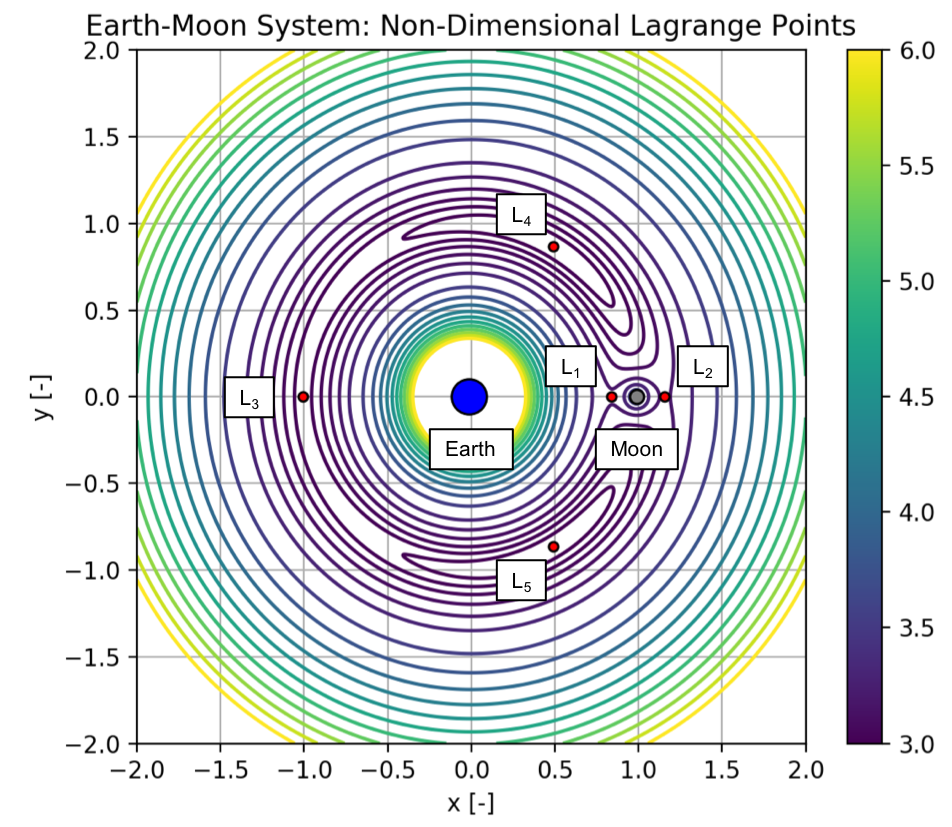
\includegraphics[width=6in]{zerovelocity_earthmoon.png}
    \caption{This figure depicts the the 5 equilibrium points and the zero-velocity curves in the non-dimensional Earth-Moon CR3BP system.}
    \label{f:lagrange_points}
\end{figure}

%-------------------------------------------------------------------

%-------------------------------------------------------------------
\subsection{Equilibrium Point Stability}
In this section, a planar stability analysis is performed about each Lagrange point in the Earth-Moon CR3BP. This study entails linearizing the CR3BP equations of motion about each equilibrium solution and solving for the eigenvalues at the equilibrium point. The CR3BP equations of motion can be linearized by taking a Taylor series expansion of the ODE about each equilibrium point in the system. Neglecting higher order terms, the linearized equations of motion are give by

\begin{equation}
	\label{e:lin_eom}
	\delta\begin{bmatrix}\dot{x}\\\dot{y}\\\ddot{x}\\\ddot{y}\end{bmatrix} = Df\left(x^*,y^*,\dot{x}^*,\dot{y}^*\right)\begin{bmatrix}x\\y\\\dot{x}\\\dot{y}\end{bmatrix},
\end{equation}

\noindent
where

\doublespacing
\begin{equation}
	\label{e:df_raw}
	Df\left(x,y,\dot{x},\dot{y}\right) = 
	\begin{bmatrix} 
		\frac{\partial \dot{x}}{\partial x} & \frac{\partial \dot{x}}{\partial y} & \frac{\partial \dot{x}}{\partial \dot{x}}  & \frac{\partial \dot{x}}{\partial \dot{y}} \\ 
		\frac{\partial \dot{y}}{\partial x} & \frac{\partial \dot{y}}{\partial y} & \frac{\partial \dot{y}}{\partial \dot{x}} & \frac{\partial \dot{y}}{\partial \dot{y}} \\
		\frac{\partial \ddot{x}}{\partial x} & \frac{\partial \ddot{x}}{\partial y} & \frac{\partial \ddot{x}}{\partial \dot{x}} & \frac{\partial \ddot{x}}{\partial \dot{y}} \\
		\frac{\partial \ddot{y}}{\partial x} & \frac{\partial \ddot{y}}{\partial y} & \frac{\partial \ddot{y}}{\partial \dot{x}} & \frac{\partial \ddot{y}}{\partial \dot{y}}
	\end{bmatrix}.
\end{equation}
\singlespacing

\noindent 
For the CR3BP, Equation \ref{e:df_raw} evaluates to 

\doublespacing
\begin{equation}
	\label{e:df_eval}
	Df\left(x,y,\dot{x},\dot{y}\right) = 
	\begin{bmatrix} 
		0 & 0 & 1  & 0 \\ 
		0 & 0 & 0 & 1 \\
		XX & XY & 0 & 2 \\
		YX & YY & -2 & 0
	\end{bmatrix},
\end{equation}
\singlespacing

\noindent
where

\begin{align}
	XX &= \frac{\mu - 1}{r_1^3} - \frac{\mu}{r_2^3} + \frac{3\mu\left(\mu+x-1\right)^2}{r_2^5} - \frac{3\left(\mu+x\right)^2\left(\mu-1\right)}{r_1^5} + 1 \\
	XY &= YX = \frac{3\mu y\left(\mu+x-1\right)}{r_2^5} - \frac{3y\left(\mu+x\right)\left(\mu-1\right)}{r_1^5} \\
	YY &= \frac{\mu - 1}{r_1^3} - \frac{\mu}{r_2^3} + \frac{3\mu y^2}{r_2^5} - \frac{3y^2\left(\mu-1\right)}{r_1^5} + 1.
\end{align}

\noindent
By evaluating the matrix given in Equation \ref{e:df_eval} at the equilibrium points and finding the resulting eigenvalues of the matrix, the stability of that point can be ascertained.

\subsubsection{L$_1$, L$_2$, and L$_3$ Stability}
It was visually shown in Figure \ref{f:lagrange_points} that L$_1$, L$_2$, and L$_3$ were saddle points. By plugging in the locations of the equilibrium points given in Table \ref{t:lagrange_points} along with the Earth-Moon three-body parameter ($\mu = 0.012155$), this claim can be mathematically validated. 

\subsubsection*{L$_1$}
The evaluated $Df$ matrix for the L$_1$ Lagrange point is given by

\doublespacing
\begin{equation}
	\label{e:df_eval_L1}
	Df|_{L_1} = 
	\begin{bmatrix} 
		0 & 0 & 1  & 0 \\ 
		0 & 0 & 0 & 1 \\
		11.2955 & 0 & 0 & 2 \\
		0 & -4.1478 & -2 & 0
	\end{bmatrix},
\end{equation}
\singlespacing

\noindent
where

\begin{equation}
	\label{e:evals_L1}
	\lambda_{1,2} = \pm 2.9321 \text{ and } \lambda_{3,4} = \pm i2.3344.
\end{equation}

\noindent
As Equation \ref{e:evals_L1} shows, the L$_1$ equilibrium point has a positive, real eigenvalue that results in a dynamically unstable saddle point. Small departures from the equilibrium will grow exponentially with a time constant of $\tau = 1/real(\lambda_{3,4}) = 0.4284$. Re-dimensionalizing this value by the rotation rate of the Earth-Moon system ($\omega=2.665\times10^{-6}$ rad/sec) results in a time constant of $\tau\approx1.86$ days. In other words, a satellite parked at L$_1$ will wander off after a few days unless course corrections are made.

\subsubsection*{L$_2$}
The evaluated $Df$ matrix for the L$_2$ Lagrange point is given by

\doublespacing
\begin{equation}
	\label{e:df_eval_L2}
	Df|_{L_2} = 
	\begin{bmatrix} 
		0 & 0 & 1  & 0 \\ 
		0 & 0 & 0 & 1 \\
		7.3807 & 0 & 0 & 2 \\
		0 & -2.1903 & -2 & 0
	\end{bmatrix},
\end{equation}
\singlespacing

\noindent
where

\begin{equation}
	\label{e:evals_L2}
	\lambda_{1,2} = \pm 2.1586 \text{ and } \lambda_{3,4} = \pm i1.8626.
\end{equation}

\noindent
Similarly to the L$_1$ point, the L$_2$ Lagrange point has a positive, real eigenvalue that results in a dynamically unstable saddle point. The re-dimensionalized L$_2$ time constant is $\tau\approx2.33$ days. 

\subsubsection*{L$_3$}
The evaluated $Df$ matrix for the L$_3$ Lagrange point is given by

\doublespacing
\begin{equation}
	\label{e:df_eval_L3}
	Df|_{L_3} = 
	\begin{bmatrix} 
		0 & 0 & 1  & 0 \\ 
		0 & 0 & 0 & 1 \\
		3.0214 & 0 & 0 & 2 \\
		0 & -0.0107 & -2 & 0
	\end{bmatrix},
\end{equation}
\singlespacing

\noindent
where

\begin{equation}
	\label{e:evals_L3}
	\lambda_{1,2} = \pm 0.1779 \text{ and } \lambda_{3,4} = \pm i1.0104.
\end{equation}

\noindent
Once again, the evaluated $Df$ matrix has a positive, real eigenvalue resulting in the L$_3$ Lagrange point being unstable. The re-dimensionalized L$_3$ time constant is $\tau\approx4.30$ days.

\subsubsection{L$_4$ and L$_5$ Stability}
The stability analysis of the L$_4$ and L$_5$ Lagrange points yields a surprise. While these points correspond to local maxima of the total potential, they are stable due to a ``Coriolis'' force. Initially, a mass situated near L$_4$ or L$_5$ will tend to slide down the potential, but as it does, it picks up speed sending it into an orbit around the equilibrium point. To prove this, the evaluated $Df$ matrix for the L$_4$ and L$_5$ Lagrange points is given by

\doublespacing
\begin{equation}
	\label{e:df_eval_L45}
	Df|_{L_4,5} = 
	\begin{bmatrix} 
		0 & 0 & 1  & 0 \\ 
		0 & 0 & 0 & 1 \\
		0.7500 & \pm1.2675 & 0 & 2 \\
		\pm1.2675 & 2.2500 & -2 & 0
	\end{bmatrix},
\end{equation}
\singlespacing

\noindent
where

\begin{equation}
	\label{e:evals_L45}
	\lambda_{1,2} = \pm i0.9545 \text{ and } \lambda_{3,4} = \pm i0.2983.
\end{equation}

\noindent
As Equation \ref{e:evals_L45} shows, the L$_4$ and L$_5$ equilibrium points have purely imaginary eigenvalues in the Earth-Moon system resulting in Lyapunov stability. However, this is not always the case for a three body system. In order for the L$_4$ and L$_5$ Lagrange points to be stable, the primary masses of the system have to satisfy the follow \textbf{inequality \cite{ScheersBook}}

\begin{equation}
	\frac{m_1}{m_2} > \frac{25+\sqrt{621}}{2}\approx24.96.
\end{equation}

\noindent
For reference, $m_1/m_2=81.27$ for the Earth-Moon system. Now that the Earth-Moon equilibrium points have been identified, numerical methods can be used to generate families of periodic orbits about the points.
%-------------------------------------------------------------------

%-------------------------------------------------------------------
\subsection{Periodic Orbits}
The solution flow of a dynamical system is often times denoted $\bm{x}\left(t\right)=\bm{\varphi}\left(t;\bm{x}_0\right)$ with initial condition $\bm{x}\left(t_0\right)=\bm{\varphi}\left(t_0;\bm{x}_0\right)$. A periodic orbit is a solution of the system such that $\bm{\varphi}\left(t+T;\bm{x}_0\right) = \bm{\varphi}\left(t;\bm{x}_0\right)$ for all $t$ where $T>0$ is the period of the orbit. Lyapunov's Center Theorem then states that for a system with an integral of motion (the Jacobi constant in the case of the CR3BP), if $Df\left(\bm{x}^*\right)$ has eigenvalues $\pm i\omega, \lambda_3, \lambda_4,...,\lambda_n$, then there exists a one-parameter family of periodic orbits emanating from the equilibrium point. Furthermore, periods tend to $2\pi/\omega$ when approaching the equilibrium point along the \textbf{family \cite{MeyerandHallBook}}. Using this knowledge, one of the most straightforward methods used to solve for periodic orbit families is to make educated guesses at individual periodic orbit initial conditions and then use a single shooter algorithm to correct them. 

\subsubsection{Family Finding Algorithm}
The family finding algorithm (FFA) begins by determining the dynamical system's fundamental matrix $\Phi\left(t,t_0\right)$. In a system as complicated as the CR3BP, $\Phi$ must be computed numerically through the following differential equation

\begin{equation}
	\dot{\Phi}=Df\left(\bm{x}\right)\Phi \text{ with } \Phi\left(t_0,t_0\right)=\mathcal{I}.
\end{equation}

\noindent
The full dynamics matrix $Df$, which was touched on in Equation \ref{e:df_eval}, is given by

\doublespace
\begin{equation}
	\label{e:df_full}
	Df = \begin{bmatrix}
		0_{3\times3} & \mathcal{I}_{3\times3} \\
		\Omega_{i,j} & V
	\end{bmatrix}
\end{equation}
\singlespace

\noindent
where, $0$ is a $3\times3$ zero matrix, $\mathcal{I}$ is a $3\times3$ identity matrix, $V$ is given by

\begin{equation}
	V = \begin{bmatrix}
		0 & 2 & 0 \\
		-2 & 0 & 0 \\
		0 & 0 & 0
	\end{bmatrix},
\end{equation}

\noindent
and $\Omega_{i,j}$ is a $3\times3$ matrix of second order partial derivatives ($\Omega_{i,j}$ = $\Omega_{j,i}$) given by

\begin{align}
	\Omega_{x,x} &= \frac{\partial\ddot{x}}{\partial x} = \frac{\mu - 1}{r_1^3} - \frac{\mu}{r_2^3} + \frac{3\mu\left(\mu+x-1\right)^2}{r_2^5} - \frac{3\left(\mu+x\right)^2\left(\mu-1\right)}{r_1^5} + 1 \\
	\Omega_{y,y} &= \frac{\partial\ddot{y}}{\partial y} = \frac{\mu - 1}{r_1^3} - \frac{\mu}{r_2^3} + \frac{3\mu y^2}{r_2^5} - \frac{3y^2\left(\mu-1\right)}{r_1^5} + 1 \\
	\Omega_{z,z} &= \frac{\partial\ddot{z}}{\partial z} = \frac{\mu - 1}{r_1^3} - \frac{\mu}{r_2^3} + \frac{3\mu z^2}{r_2^5} - \frac{3z^2\left(\mu-1\right)}{r_1^5} \\
	\Omega_{x,y} &= \frac{\partial\ddot{x}}{\partial y} = \frac{3\mu y\left(\mu+x-1\right)}{r_2^5} - \frac{3y\left(\mu+x\right)\left(\mu-1\right)}{r_1^5} \\
	\Omega_{y,z} &= \frac{\partial\ddot{y}}{\partial z} = \frac{3\mu z\left(\mu+x-1\right)}{r_2^5} - \frac{3z\left(\mu+x\right)\left(\mu-1\right)}{r_1^5}\\
	\Omega_{z,x} &= \frac{\partial\ddot{z}}{\partial x} = \frac{3\mu yz}{r_2^5} - \frac{3yz\left(\mu-1\right)}{r_1^5}.
\end{align}

\noindent
Using the aforementioned Lyapunov Center Theorem, the FFA is initiated by perturbing the equilibrium point of interest in the direction of a center manifold (purely imaginary eigenvalue) by a small amount ($\epsilon < 1\times10^{-4}$). This results in the ``smallest'' periodic orbit around the equilibrium point. The period of the orbit is then determined by the value of the eigenvalue ($T=2\pi/\lambda$). To continue the FFA, future periodic orbit initial conditions ($\bm{x}_0, T$) are calculated by adding small perturbations to the previous periodic orbit initial conditions ($\tilde{\bm{x}}_0, \tilde{T}$) in the orbit tangent direction ($\tilde{\bm{x}}_0^{\prime}, \tilde{T}^{\prime}$). This update is mathematically shown as follow

\begin{align}
	\bm{x}_0 &= \tilde{\bm{x}}_0 + \Delta s\tilde{\bm{x}}_0^{\prime} \\
	T &= \tilde{T} + \Delta s\tilde{T}^{\prime},
\end{align}

\noindent
where $\Delta s$ is the step size between the original periodic orbit and the new periodic orbit and the orbit tangent direction is approximated by the change in the initial conditions between two previous orbits. In order to insure that the new periodic orbit is part of the periodic orbit family, two important constraints must be satisfied. The first constraint, known as the Poincar\'{e} phase condition, which assumes that a periodic orbit in the family has already been computed, states that 

\begin{equation}
	<\bm{x}_0 - \tilde{\bm{x}}_0, \bm{f}\left(\tilde{\bm{x}}_0\right)> = 0,
\end{equation}

\noindent
where $\bm{f}\left(\bm{x}\right)$ are the dynamics of the CR3BP evaluated at some state. The second constraint, known as the pseudo-arclength continuation constraint, which assumes that a periodic orbit in the family and an approximation of the tangent to the solution family has already been computed, states that

\begin{equation}
<\bm{x}_0 - \tilde{\bm{x}}_0, \tilde{\bm{x}}_0^{\prime}> + \left(T-\tilde{T}\right)\tilde{T}^{\prime} = \Delta s.
\end{equation}

\noindent
Using these constraints, a system of equations for the FFA is given by

\doublespace
\begin{equation}
	\label{e:ffa_constraints}
	\begin{bmatrix}
	\bm{\varphi}\left(T;\bm{x}_0\right) - \bm{x}_0 \\
	<\bm{x}_0 - \tilde{\bm{x}}_0, \bm{f}\left(\tilde{\bm{x}}_0\right)> \\
	<\bm{x}_0 - \tilde{\bm{x}}_0, \tilde{\bm{x}}_0^{\prime}> + \left(T-\tilde{T}\right)\tilde{T}^{\prime} - \Delta s
	\end{bmatrix} = \bm{F}\left(\bm{x}_0, T\right) = \bm{0},
\end{equation}
\singlespace

\noindent
where $\bm{x}_0$ and $T$ are unknowns. This system of equations is then solved using a single shooter \textbf{algorithm \cite{SingleShooter}} which is given in the form

\doublespace
\begin{equation}
	\label{e:singleshooter}
	\begin{bmatrix}
	\Phi\left(T\right) - \mathcal{I}_{n\times n} & \bm{f}\left(\bm{x}\left(T\right)\right) \\
	\dot{\tilde{\bm{x}}}_0 & 0 \\
	\tilde{\bm{x}}_0^{\prime} & \tilde{T}^{\prime} \\
	\end{bmatrix} \begin{bmatrix}
	\delta\bm{x}_0 \\
	\delta T
	\end{bmatrix} = -\bm{F}\left(\bm{x}_0, T\right),
\end{equation}
\singlespace

\noindent
where $\delta\bm{x}_0$ and $\delta T$ are updates to the initial conditions of the new periodic orbit. Since the single shooter algorithm uses a first-order Newton-Raphson method, Equation \ref{e:singleshooter} is iterated until convergence. Furthermore, since this system is overdetermined ($n+2$ equations and $n+1$ unknowns), a pseudo-inverse is used when solving for $\delta\bm{x}_0$ and $\delta T$. An example of the single shooter algorithm correcting a periodic orbit is shown in Figure \ref{f:singleshooter}. Using this FFA, a periodic orbit family can be calculated with minimal a priori knowledge for as many number of periodic orbits as desired. 

\begin{figure}[H]
    \centering
    \includegraphics[width=6in]{po_corrected.png}
    \caption{This figure shows the single shooter algorithm correcting a periodic orbit. Figure (a) shows the uncorrected orbit, and Figure (b) shows the correct orbit.}
    \label{f:singleshooter}
\end{figure}

\subsubsection{Orbit Families}
In 1892, Poincar\'{e} showed that an infinite number of periodic solutions exist in the three-body problem. These solutions come in a variety of forms that include planar Lypaunov periodic orbits, 3-dimensional clamshell orbits, 3-dimensional halo orbits, and many others. All of these periodic orbit solutions intersect and merge with one another through complex interactions and bifurcations. Using the previously described FFA, all of these periodic orbit families can be cataloged. Figure \ref{f:lagrange_points} shows an example of planar Lypaunov periodic orbit families calculated about each of the five Lagrange points. Additionally, Figure \ref{f:clamshell_po} shows 3-dimensional clamshell orbits about L$_1$. 

\begin{figure}[H]
    \centering
    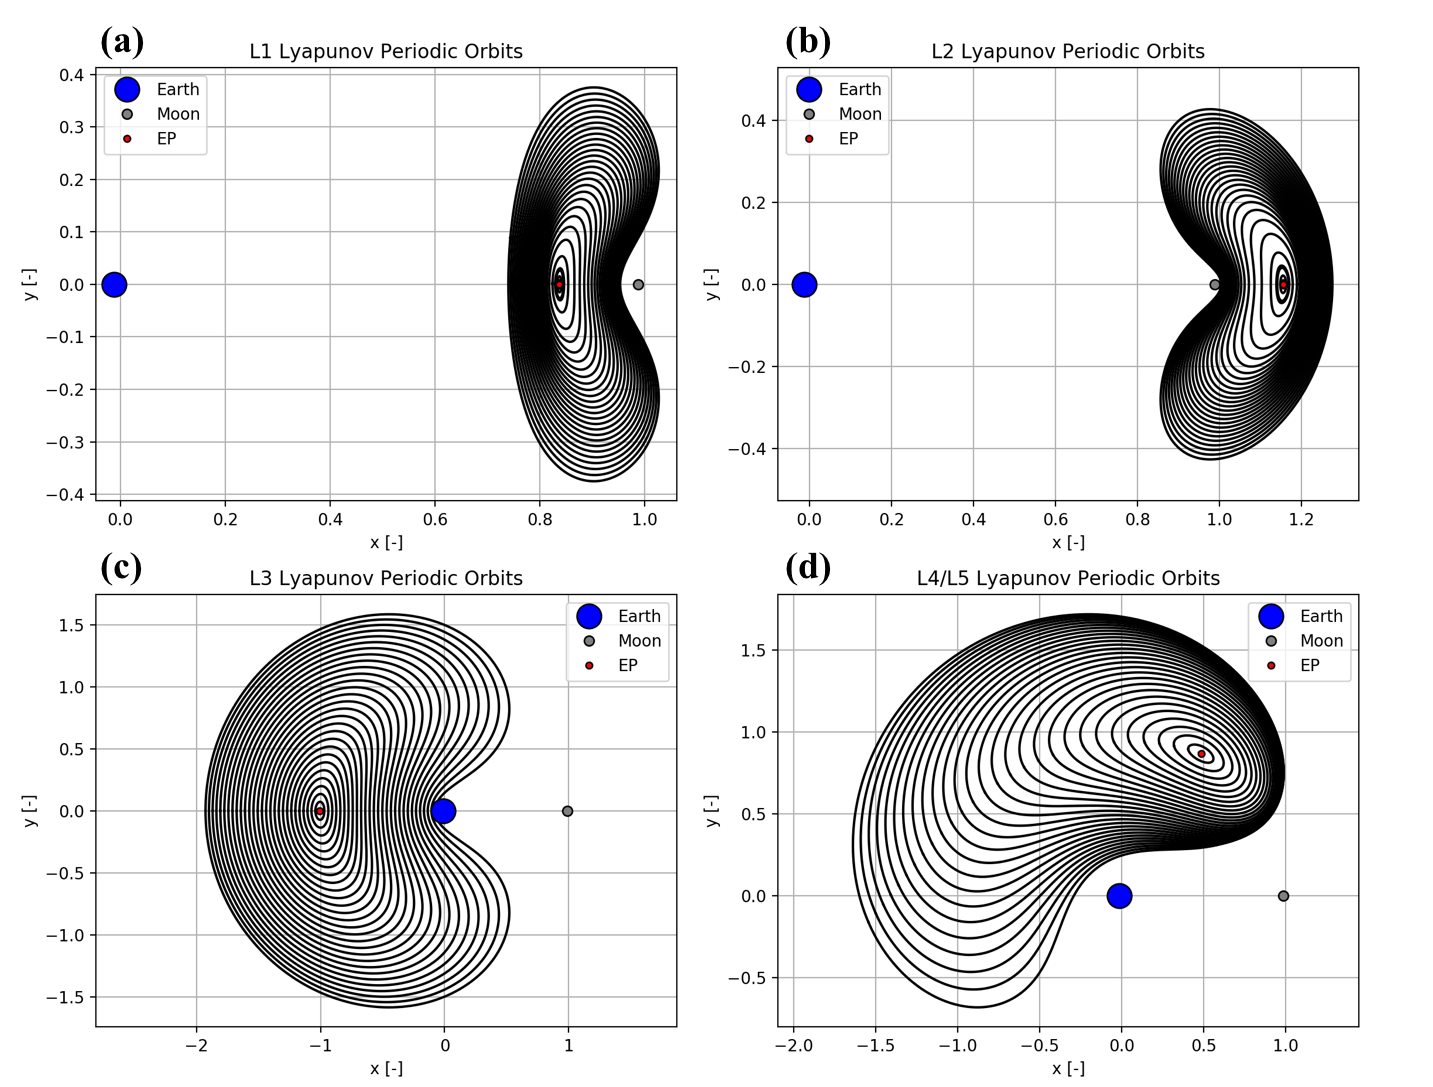
\includegraphics[width=\textwidth]{lyapunov_po_comb.png}
    \caption{This figure shows planar Lypaunov periodic orbit families about each of the five Lagrange points. Figure (a) shows orbits about L$_1$, Figure (b) shows orbits about L$_2$, Figure (c) shows orbits about L$_3$, Figure (d) shows orbits about L$_{4,5}$.}
    \label{f:lyapunov_po}
\end{figure}

\begin{figure}[H]
    \centering
    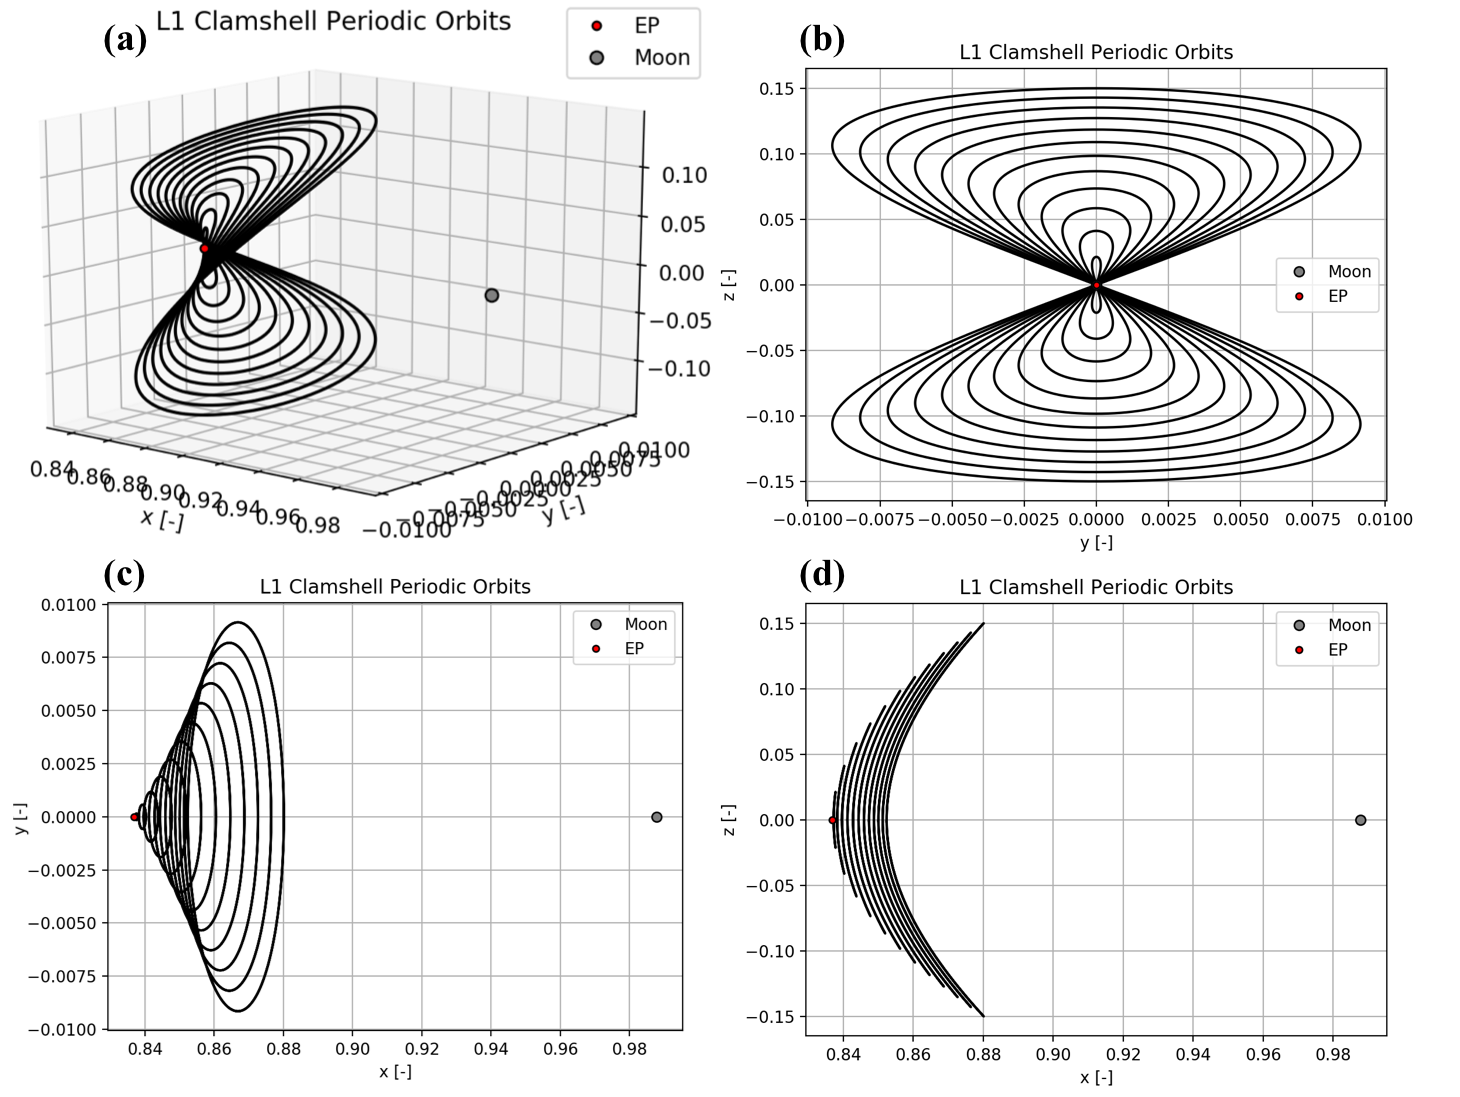
\includegraphics[width=\textwidth]{L1_clamshell_comb.png}
    \caption{This figure shows a family of 3-dimensional clamshell orbits about L$_1$.}
    \label{f:clamshell_po}
\end{figure}

%-------------------------------------------------------------------

%-------------------------------------------------------------------
\subsection{Periodic Orbit Stability and Manifolds}
In dynamical systems, periodic orbits are invariant sets (i.e., for each $x \in \Lambda, \varphi\left(t;x\right)\in\Lambda$ for any $t$), and as such, their stability can be discussed. In order to determine the stability of a periodic orbit, the eigenvalues of the orbit's Monodromy matrix, which is defined as a periodic orbit's fundamental matrix evaluated after one period $T$ (i.e., $M=\Phi\left(t_0+T,t_0\right)$), need to be analyzed. For the CR3BP, the Monodromy matrix has six eigenvalues and six corresponding eigenvectors. Since $M$ is symplectic, the eigenvalues will come in 3 pairs with one of the pairs always being equal to 1. The relationship between the eigenvalues is as follows

\begin{align}
	\lambda_1 &= \frac{1}{\lambda_2}\\
	\lambda_3 &= \frac{1}{\lambda_4}\\
	\lambda_5 &= \lambda_6 = 1.
\end{align}

\noindent
The eigenvalues of the Monodromy matrix determine the effect of small perturbations on a periodic orbit. If the real components of the eigenvalue are between -1 and 1, a perturbation in that direction will exponentially decay and the orbit is considered stable. Conversely, if the real components are outside of -1 and 1, a perturbation in that direction will exponentially grow and the orbit is considered unstable. If the eigenvalue is only imaginary, then the perturbation will oscillate about the original state after each period. Finally, if the eigenvalues are equal to 1, the perturbation does not grow or decay (unit eigenvalues are therefore normally ignored).

In order to map a stable or unstable manifold of a periodic orbit, the initial conditions of the orbit must be perturbed in the direction of the manifold (i.e., in the direction of the eigenvector corresponding to the manifold of interest). To fully map these manifolds, the periodic orbit needs to be perturbed at many points along its trajectory. This is accomplished by using the fundamental matrix to map the original stable or unstable eigenvector $\bm{v}^{S,U}$ from $M$ to any point on the periodic orbit (i.e., $\bm{v}_i^{S,U}=\Phi\left(t_i,t_0\right)\bm{v}^{S,U}$). The periodic orbit is then perturbed by a small amount ($\epsilon < 1\times10^{-4}$) in the direction of the mapped eigenvector (i.e., $\bm{x}_{i}^{S,U}=\bm{x}_{i}\pm\epsilon|\bm{v}_i^{S,U}|$). To see the shape of each manifold, the unstable manifold is then propagated forward in time while the stable manifold is propagated backwards in time. Each periodic orbit in the CR3BP has both interior and exterior stable and unstable manifolds depending on the sign of the applied perturbation. Figure \ref{f:manifolds} shows the exterior stable (green) and unstable (red) manifolds of a L$_2$ Lyapunov periodic orbit. As Figure \ref{f:manifolds} shows, these manifolds are intricate structures that extend far into the CR3BP phase space. 

\begin{figure}[H]
    \centering
    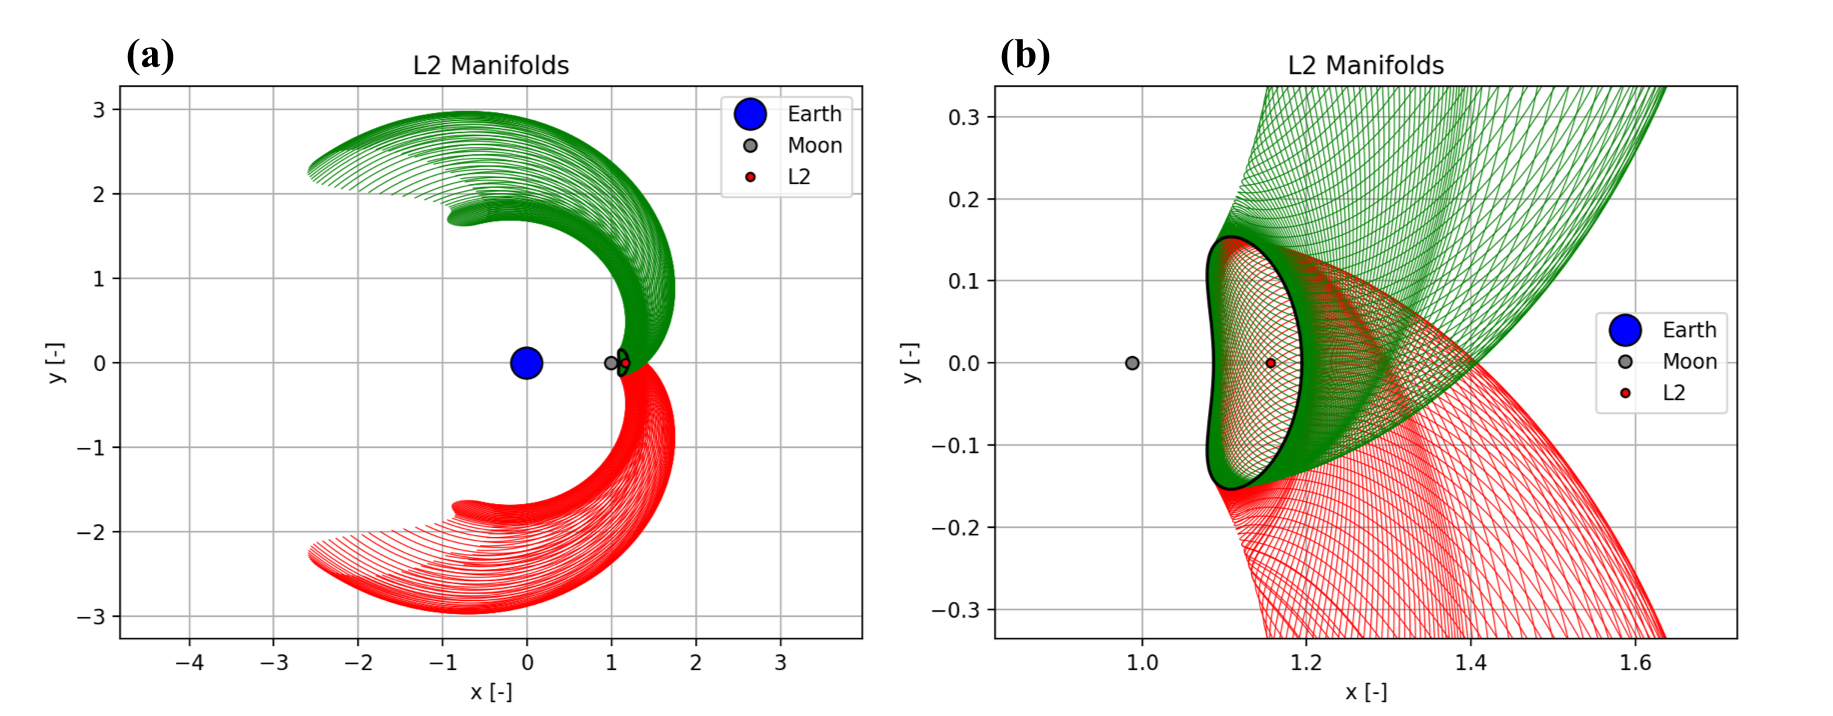
\includegraphics[width=\textwidth]{manifold_comb.png}
    \caption{This figure shows the exterior stable (green) and unstable (Red) manifolds of a L$_2$ Lyapunov periodic orbit.}
    \label{f:manifolds}
\end{figure}
%-------------------------------------------------------------------

%-------------------------------------------------------------------
\subsection{Poincar\'{e} Sections and Homoclinic Orbits}
In a dynamical system, an orbit $\Gamma$ is homoclinic if each $x\in\Gamma$ is both forward and backwards asymptotic to the same invariant set $\Lambda$. In other words, this means that for any $x\in\Gamma$ as $t\rightarrow\pm\infty$, $x\rightarrow\Lambda$. In order for this to occur, a homoclinic orbit must be contained in the intersection of the stable $W^S\left(\Lambda\right)$ and unstable $W^U\left(\Lambda\right)$ manifolds of the invariant set (i.e., $\Gamma\subset W^S\left(\Lambda\right)\cap W^U\left(\Lambda\right)$). Classically, a mathematical technique known as a Poincar\'{e} section is used to find the intersection of $W^S\left(\Lambda\right)$ and $W^U\left(\Lambda\right)$. 

In the CR3BP, a Poincar\'{e} section, which is defined as lower dimensional surface of section that is transverse to the flow of a dynamical system, is used to map the characteristics of the stable ($W^S\left(\Lambda\right)$) and unstable ($W^U\left(\Lambda\right)$) manifolds of a periodic orbit ($\Lambda$). Figure \ref{f:poincare} shows an example of a Poincar\'{e} section for two different periodic orbits about the L$_2$ Lagrange point. In the CR3BP, a common Poincar\'{e} section for the L$_2$ Lagrange point is the surface $y=0$ and $x<0$. This surface is indicated in Figure \ref{f:poincare}a and Figure \ref{f:poincare}b as the thick black line at $y=0$. In order to find the intersection of the stable (green) and unstable (red) manifolds of the periodic orbit, both manifolds are propagated (as described in the previous section) to the Poincar\'{e} section where their $x$-position and $x$-velocity are recorded. The position and velocity of both manifolds are then plotted against one another, as shown in Figure \ref{f:poincare}c and Figure \ref{f:poincare}d, to determine if there is any intersection points between the two manifolds (i.e., $\Gamma\subset W^S\left(\Lambda\right)\cap W^U\left(\Lambda\right)$). In other words, the intersections of the stable and unstable manifolds on the Poincar\'{e} section represent the location of homoclinic orbits. A careful inspection of Figure \ref{f:poincare}d reveals that there are eight intersection points in between $W^S\left(\Lambda\right)$ and $W^U\left(\Lambda\right)$ corresponding to eight different homoclinic orbits for the periodic orbit in question. However, it is important to note that not every periodic orbit has homoclinic trajectories, as Figure \ref{f:poincare}c shows. 

\begin{figure}[H]
    \centering
    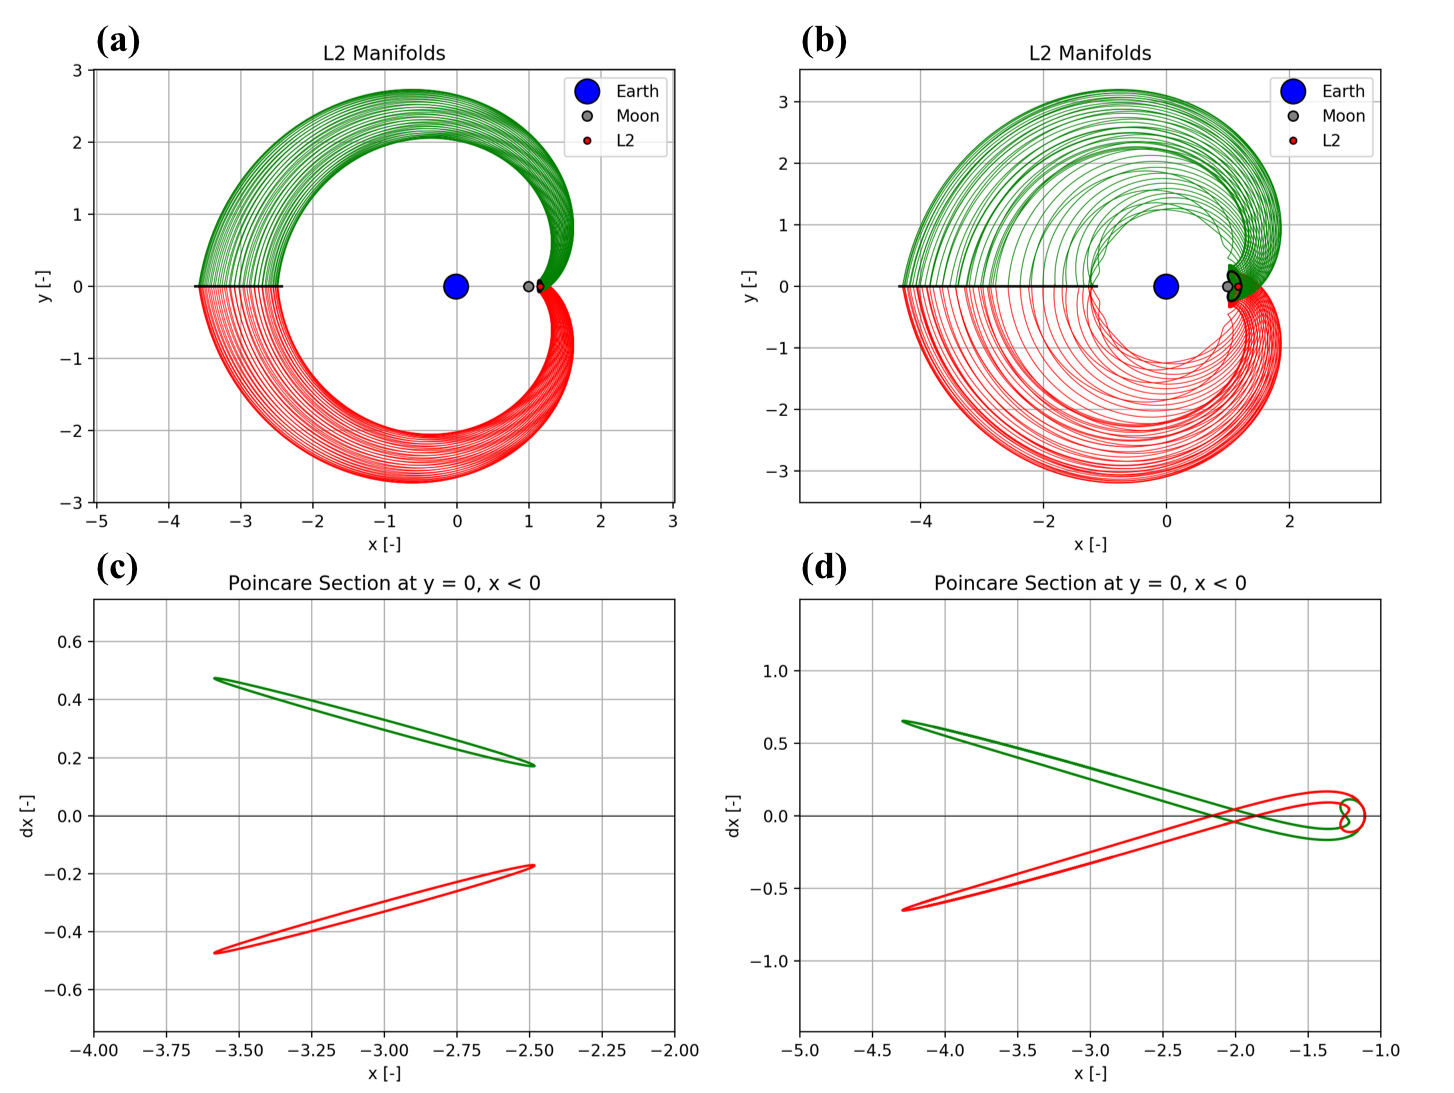
\includegraphics[width=\textwidth]{poincare_comb.png}
    \caption{This figure shows the construction of a Poincar\'{e} section for two different periodic orbits about the L$_2$ Lagrange point.}
    \label{f:poincare}
\end{figure}

Figure \ref{f:sym_homo}a takes a closer look at the intersection of the stable and unstable manifolds the periodic orbit shown in Figure \ref{f:poincare}b. As Figure \ref{f:sym_homo}a shows, there are four intersection points located on the line $\dot{x}=0$ and four points located off of line $\dot{x}=0$. The manifold intersection points that lie on the line $\dot{x}=0$ represent symmetric homoclinic orbits, whereas the points that lie off the line represent asymmetric homoclinic orbits. An example of these different types of orbits can be seen in Figure \ref{f:sym_homo}b and Figure \ref{f:asym_homo}b, respectively. As Figure \ref{f:sym_homo}b and Figure \ref{f:asym_homo}b show, the two homoclinic orbits depart from the periodic orbit on the unstable manifold (red) and return to the periodic orbit on the stable manifold (green). Finding the exact initial conditions for homoclinic orbits is quite difficult due to the sensitivity of initial conditions of the CR3BP, but we did it!

\begin{figure}[H]
    \centering
    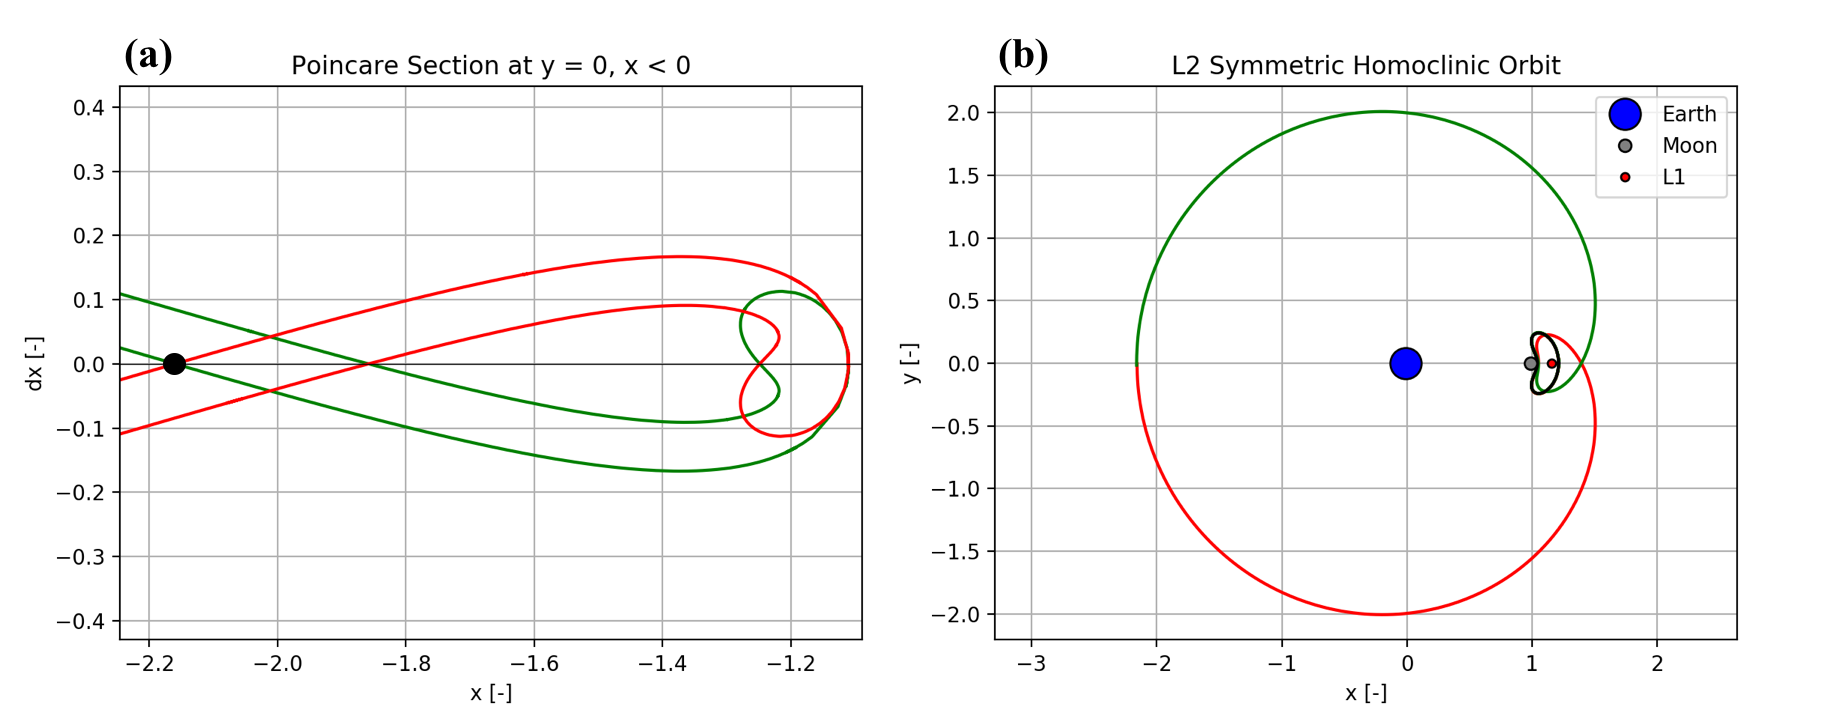
\includegraphics[width=\textwidth]{sym_homo_comb.png}
    \caption{This figure shows a symmetric homoclinic orbit about the L$_2$ Lagrange point. The grey dot in Figure (a) represents the homoclinic orbit investigated.}
    \label{f:sym_homo}
\end{figure}

\begin{figure}[H]
    \centering
    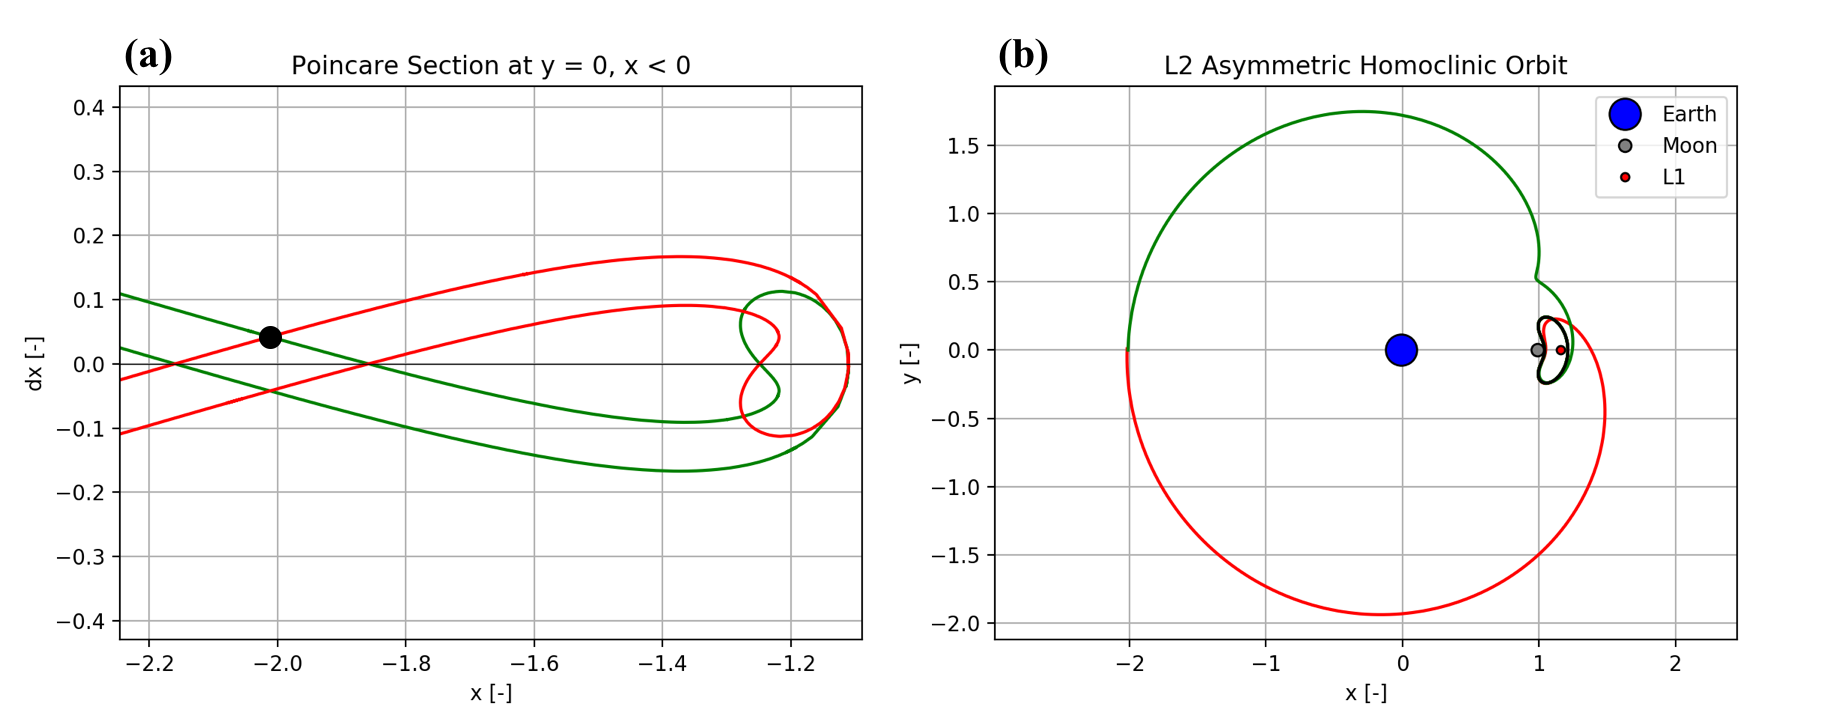
\includegraphics[width=\textwidth]{asym_homo_comb.png}
    \caption{This figure shows a asymmetric homoclinic orbit about the L$_2$ Lagrange point. The grey dot in Figure (a) represents the homoclinic orbit investigated.}
    \label{f:asym_homo}
\end{figure}

%-------------------------------------------------------------------

%-------------------------------------------------------------------
\section{Conclusion}
\begin{itemize}
	\item \color{red}{Homoclinic orbits are cool/interesting, but for spacecraft applications they aren't very useful; Heteroclinic orbits are useful fa show}\color{black}
\end{itemize}

\begin{figure}[H]
    \centering
    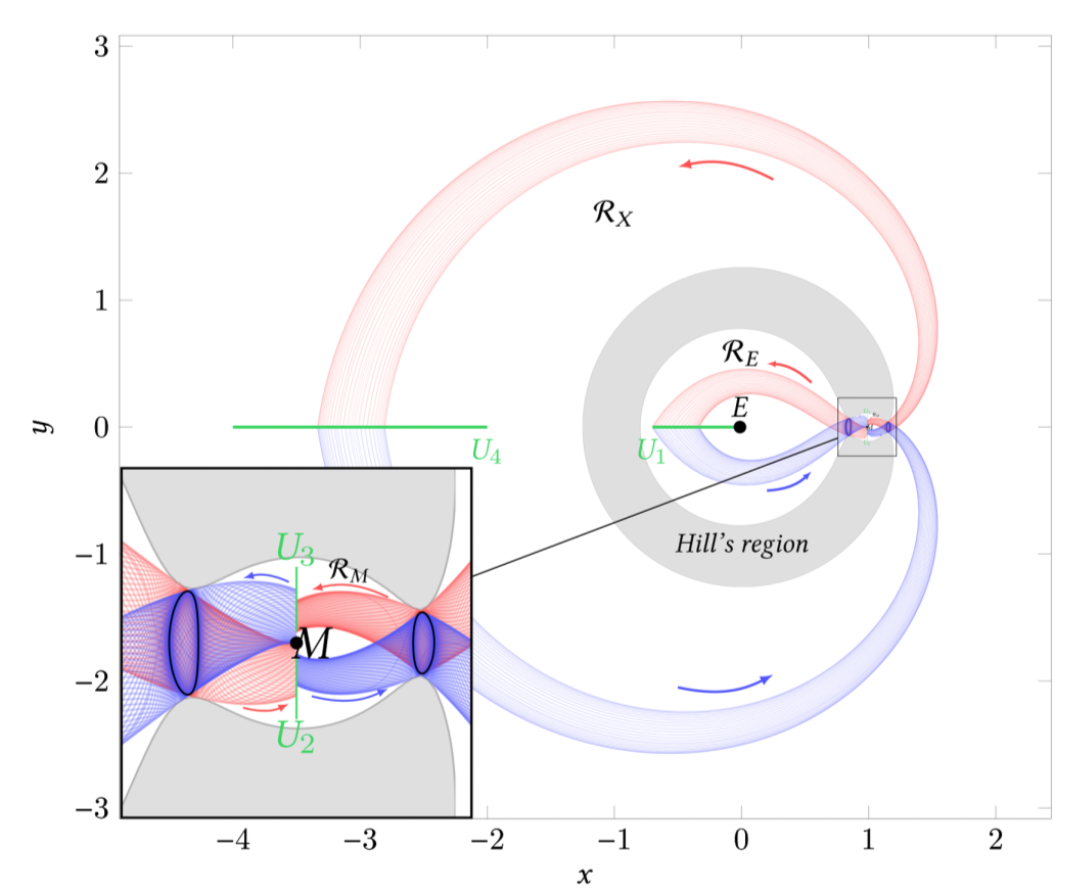
\includegraphics[width=5in]{interior_exterior.png}
    \caption{This figure shows a full mapping of the interior and exterior, stable and unstable, L$_1$ and L$_2$ Lagrange points to appropriate Poincar\'{e} sections \cite{KoonLoMarsdenRoss2011}.}
    \label{f:interior_exterior}
\end{figure}

%===================================================================
\newpage
\bibliographystyle{plain}
\bibliography{../bibliography/appm5460.bib}

\end{document}  